%====================================================================================
\section[Test]{Test de heterocedasticidad}
%====================================================================================

\begin{frame}{Probando heterocedasticidad}
	Básicamente, existen 2 pruebas para comprobar la presencia de heterocedasticidad: La prueba de White y la prueba de Breush-Pagan
		\begin{itemize}
			\item La prueba de White considera los efectos lineales y no lineales como fuente de heterocedasticidad.
			\item El de Breusch Pagan solo considera efectos lineales e incluye otras variables exógenas.
		\end{itemize}
	¿Cuál es la hipóteis nula para esas pruebas? \textit{Respuesta}:
		\begin{center}
			$H_0$ : Homocedasticidad\\
			$H_a$ : Heterocedasticidad
		\end{center}
\end{frame}
%---------------------------------------------------
\begin{frame}{Probando heterocedasticidad}
	\begin{itemize}
		\item Esencialmente lo que se quiere probar es \\
				$H_{o}:Var(u/x_{1},x_{2},...,x_{k})=\sigma^2$
		\pause
		\item En virtud que se asume $E(u/x)=0$, $Var(u/x)=E(u^2/x)$, así la hipótesis nula de homocedasticidad es equivalente a:\\
		$H_{o}:E(u^{2}/x_{1},x_{2},...,x_{k})=E(u^{2})=\sigma^2$
		\pause
		\item Para probar la violación del supuesto de homocedasticidad se busca probar que $E(u^{2})$ se relaciona con una o más variables explicativas.
		\pause
		\item Así, para $u^{2}=\delta_{0}+\delta_{1}x_{1}+...+\delta_{k}x_{k}+v$ ello implica probar $H_{o}:\delta_{1}=...=\delta_{k}=0$
	\end{itemize}
\end{frame}

%------------------------------------------------------------------------------------
\subsection{Test de Breusch-Pagan}
%------------------------------------------------------------------------------------

\begin{frame}{Diagnóstico: Test de Breusch-Pagan (1979)}
	\begin{itemize}
		\item No se observan los $u's$ pero pueden ser estimados a partir de la regresión: $\hat{u}^2$
		\pause
		\item Después de regresionar todos los residuos al cuadrado sobre todos los $x's$ se puede usar el estadístico $LM=nR^2$ que tiene una distribución $\chi_{k}$. En STATA sería:
		\pause
		\begin{enumerate}
			\item \colorbox{codegray}{\texttt{\textcolor{codeblue}{reg} y x1 x2}}
			\item \colorbox{codegray}{\texttt{\textcolor{codeblue}{predict error}, resid}}
			\item \colorbox{codegray}{\texttt{\textcolor{codeblue}{g} error2=\textcolor{codeblue}{error}*\textcolor{codeblue}{error}}}
			\item \colorbox{codegray}{\texttt{\textcolor{codeblue}{reg} error2 x1 x2}}
			\item display 1-chi2(k,b) -(k es el número de variables y b es igual N°Obs*R2)-
		\end{enumerate}
		\pause
		\item Si el valor $p$ es lo suficientemente pequeño, es decir, si se halla por debajo del nivel de significancia elegido, entonces rechazamos la hipótesis nula de homocedasticidad.
	\end{itemize}
\end{frame}
%---------------------------------------------------
\begin{frame}{Resumen: Test de Breusch-Pagan}
	\textbf{Pasos:}
	\begin{enumerate}
		\item Conseguir los residuos ($\hat{u}$) y elevarlos al cuadrado ($\hat{u}^2$).
		\item Ejecutar una regresión de $\hat{u}^2$ en variables sospechosas (puede incluir regresores u otras variables no incluidas en el regresión principal).
			$$\hat{u}^2 = \delta_0 + \delta X_i + \gamma Z_i + \epsilon_i$$
		\item Realizar una prueba basada en la siguiente hipótesis:
			\begin{align*}
				H_0 &: \delta = 0;\enskip \gamma = 0\\
				H_a &: \textup{Al menos uno diferente de cero}
			\end{align*}
		Para probar la hipótesis nula, debe calcular el estadístico LM y contraste con valores críticos de $\chi{^2_{k-1}}$ donde $k$ es el número de parámetros a estimar en (2).
	\end{enumerate}
\end{frame}
%---------------------------------------------------
\begin{frame}{Resumen: Test de Breusch-Pagan}
	El estadístico LM se calcula de la siguiente manera:
		$$LM = \frac{SCE_{aux}}{2.\tilde{\sigma}^{4}}$$
	$SCE_{aux}$ es la suma cuadrada de las explicadas de la regresión auxiliar $\tilde{\sigma}^{4}$ es igual a $\frac{\sum \hat{u}^2}{n}$. Este estadístico es como una distribución $\chi_{k-1}^{2}$ donde $k$ es el número de parámetros a estimar en la regresión auxiliar 
\end{frame}
%%---------------------------------------------------
%\begin{frame}{Diagnóstico: incluidos los valores ajustados por MCO}
%	\textbf{Pasos}
%		\begin{enumerate}
%			\item Obtener los riduos $(\hat{u})$ y su cuadrado $(\hat{u}^{2})$
%			\item Correr la regresión de $\hat{u}^{2}$ en los valores fijos $\hat{y}$ (puede considerar las potencias de este valor ajustado).
%				$$\hat{u}^{2} = \alpha_0 +\alpha_1 \hat{y}_1+ \alpha_2 \hat{y}_1^{2}\ldots \alpha_L \hat{y}_1^{L}$$
%			\item Realizar una prueba basada en la siguiente hipótesis
%				\begin{align*}
%					H_0 & : \alpha_1 = 0; \alpha_2 = 0; \ldots; \alpha_L = 0\\
%					H_a & : \textup{al menos uno es diferente de cero}
%				\end{align*}
%			Para probar la hipótesis nula, debe calcular el estadístico $LM$ y contrastar con los valores críticos a partir de un $\chi_{k-1}^{2}$ donde $k$ es el número de parámetros a estimar en paso 2.
%		\end{enumerate}
%\end{frame}

%------------------------------------------------------------------------------------
\subsection{Test de White}
%------------------------------------------------------------------------------------

\begin{frame}{Diagnóstico: Prueba de H. White (1980)}
	\begin{itemize}
		\item Es una generalización del test de Breusch-Pagan y básicamente consiste en considerar no linealiedades en la regresión de los errores al cuadrado.
		\pause
		\item Es decir, si antes se tenía: $u^{2}=\delta_{0}+\delta_{1}x_{1}+\delta_{2}x_{2}+v$ ahora se considerará la siguiente estructura $u^{2}=\delta_{0}+\delta_{1}x_{1}+\delta_{2}x_{2}+\delta_{3}x_{1}^{2}+\delta_{4}x_{2}^{2}+\delta_{5}x_{1}x_{2}+v$
		\pause
		\item En stata sería:
			\begin{enumerate}
				\item \colorbox{codegray}{\texttt{\textcolor{codeblue}{reg} y x1 x2}}
				\item \colorbox{codegray}{\texttt{\textcolor{codeblue}{predict error},resid}}
				\item \colorbox{codegray}{\texttt{\textcolor{codeblue}{g} error2=\textcolor{codeblue}{error}*\textcolor{codeblue}{error}}}
				\item \colorbox{codegray}{\texttt{\textcolor{codeblue}{g} tem1=x1*x1}}
				\item \colorbox{codegray}{\texttt{\textcolor{codeblue}{g} tem2=x2*x2}}
				\item \colorbox{codegray}{\texttt{\textcolor{codeblue}{g} tem3=x1*x2}}
				\item \colorbox{codegray}{\texttt{\textcolor{codeblue}{reg} error2 x1 x2 tem1 tem2 tem3}}
				\item display 1-chi2(k,b) -(k en este caso es igual a 5 y b es igual N°Obs*R2)-
			\end{enumerate}
	\end{itemize}
\end{frame}
%---------------------------------------------------
\begin{frame}{Resumen: Test de White}
	\textbf{Pasos:}
		\begin{enumerate}
			\item Conseguir los residuales ($\hat{u}$) y elevarlos al cuadrado ($\hat{u}^2$).
			\item Ejecutar una regresión de $\hat{u}^2$ en todos los regresores y en sus productos cuadrados y cruzados (esa regresión es llamada la \emph{regresión auxiliar}. En el caso de 2 regresores;
					$$\hat{u}^2 = \delta_0 + \delta_1 X_1{}_i + \delta_2 X_2{}_i + \delta_3 X_1{}_i X_2{}_i + \delta_4 X^2_1{}_i + \delta_5 X^2_2{}_i + \epsilon_i$$
			\item Realizar una prueba basada en la siguiente hipótesis
				\begin{align*}
					H_0 & : \delta_1=0: \delta_2=0;\dots; \delta_{\frac{M(M+3)}{2}}=0\\
					H_a & : \textup{Al menos uno diferente de cero}
				\end{align*}
			Para probar la hipótesis nula, se debe calcular el $R^2$ y contrastar el $NR^2$ con los valores críticos de una distribución $\chi{^2_{k-1}}$ donde $k$ es el número de parámetros a estimar en el paso 2
		\end{enumerate}
\end{frame}
%------------------------------------------------------------------------------------
\subsection{Forma alternativa del Test de White}

\begin{frame}{Forma alternativa del Test de White}
	\begin{itemize}
		\item El estadístico tradicional de White tiene el problema de consumir muchos grados de libertad (con dos regresores, la regresión relevante tendría 5 explicativas; con 6 tendría 27!)
		\pause
		\item Una sugerencia es usar los valores predichos de $\hat{y}=\hat{\beta}_{0}+\hat{\beta}_{1}x_{1}+...+\hat{\beta}_{k}x_{k}$ ya que si elevamos al cuadrado se obtiene una función que depende de todos los cuadrados y productos cruzados de las variables independientes.
		\pause
		\item Es decir, se podría probar heterocedasticidad estimando la ecuación: $\hat{u}^2=\delta_{0}+\delta_{1}\hat{y}+\delta_{2}\hat{y}^2+error$. En stata sería:
		\pause
			\begin{enumerate}
				\item \colorbox{codegray}{\texttt{\textcolor{codeblue}{reg} y x1 x2}}
				\item \colorbox{codegray}{\texttt{\textcolor{codeblue}{predict} yhat,xb}}
				\item \colorbox{codegray}{\texttt{\textcolor{codeblue}{g} yhat2=yhat*yhat}}
				\item \colorbox{codegray}{\texttt{\textcolor{codeblue}{reg} error2 yhat yhat2}}
				\item display 1-chi2(2,b) -(nótese que en este caso k siempre es igual a 2 y b es igual N°Obs*R2)-
			\end{enumerate}
	\end{itemize}
\end{frame}
%----------------------------------------------------------------------------------
\subsection{Ejemplos en STATA}
%----------------------------------------------------------------------------------
\begin{frame}[fragile]{STATA}
	Consideremos los siguientes comandos para realizar pruebas de heterocedasticidad
	{\small
\begin{lstlisting}[language=Stata, numbers=none]
use "http://fmwww.bc.edu/ec-p/data/wooldridge/HPRICE1.dta", clear
regress price lotsize sqrft bdrms
//White test
estat imtest, white
//Breusch-Pagan 1
estat hettest, rhs
//Breusch-Pagan 2
estat hettest
\end{lstlisting}
}
\end{frame}
%---------------------------------------------------
\begin{frame}{STATA: Ejemplo 1}
	\begin{figure}
		\centering
		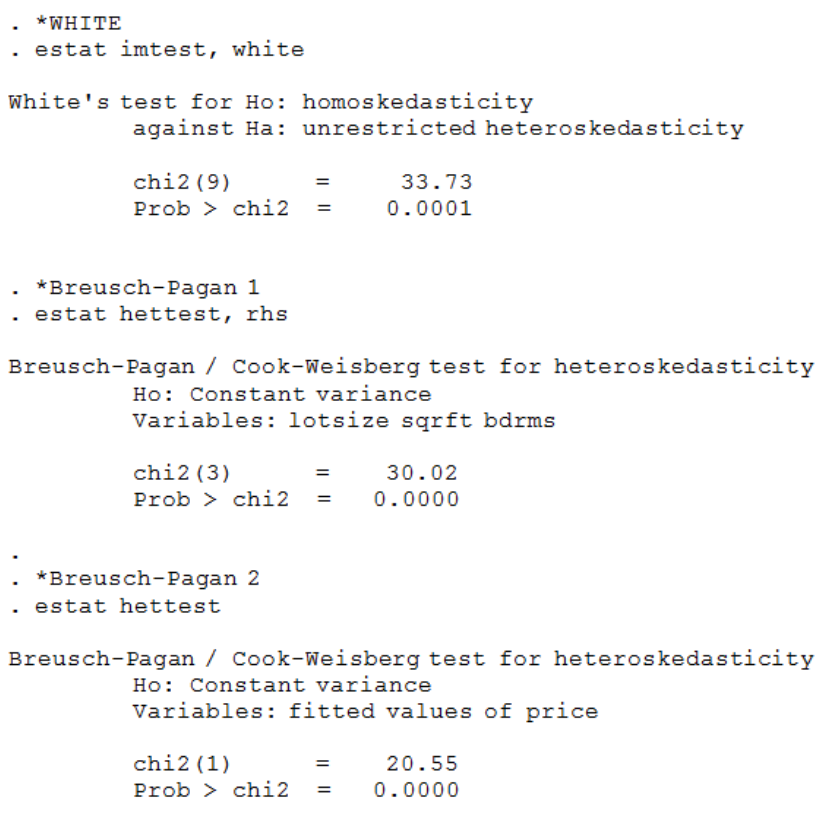
\includegraphics[scale=.37]{fig/stata1.png}
	\end{figure}
\end{frame}
%---------------------------------------------------
\begin{frame}[fragile]{STATA: Ejemplo 2}
	Consideremos el siguiente conjunto de datos (Fuente: Cameron y Trivelli dataset)
{\small
\begin{lstlisting}[language=Stata, numbers=none]
use "http://econweb.rutgers.edu/frojas/teaching/
undergraduate/mus03data.dta", clear
regress ltotexp suppins phylim actlim totchr age female income
\end{lstlisting}
}
	\begin{figure}
		\centering
		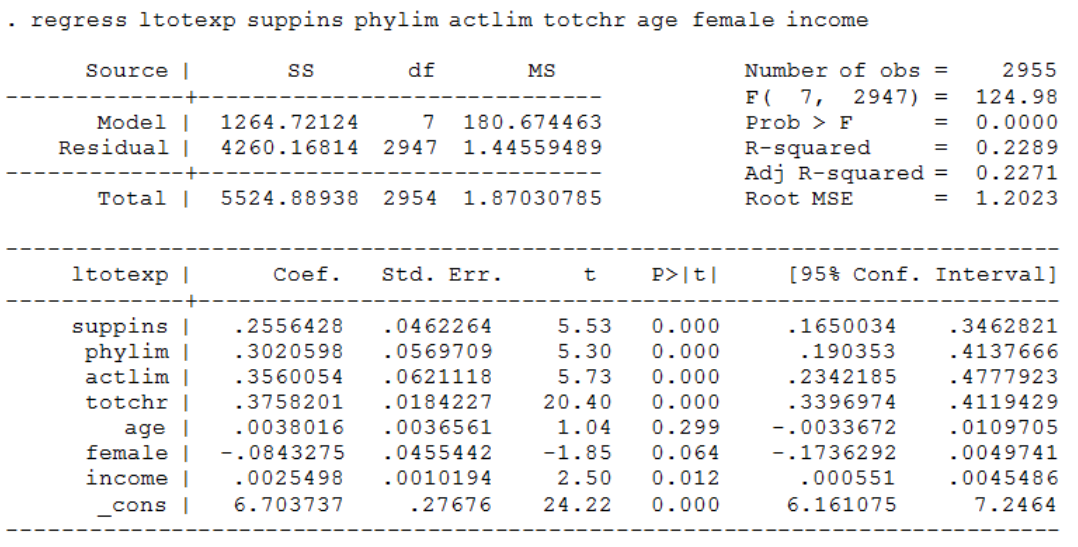
\includegraphics[scale=.33]{fig/stata2a.png}
	\end{figure}
\end{frame}
%---------------------------------------------------
\begin{frame}{STATA: Ejemplo 2}
	\begin{figure}
	\centering
	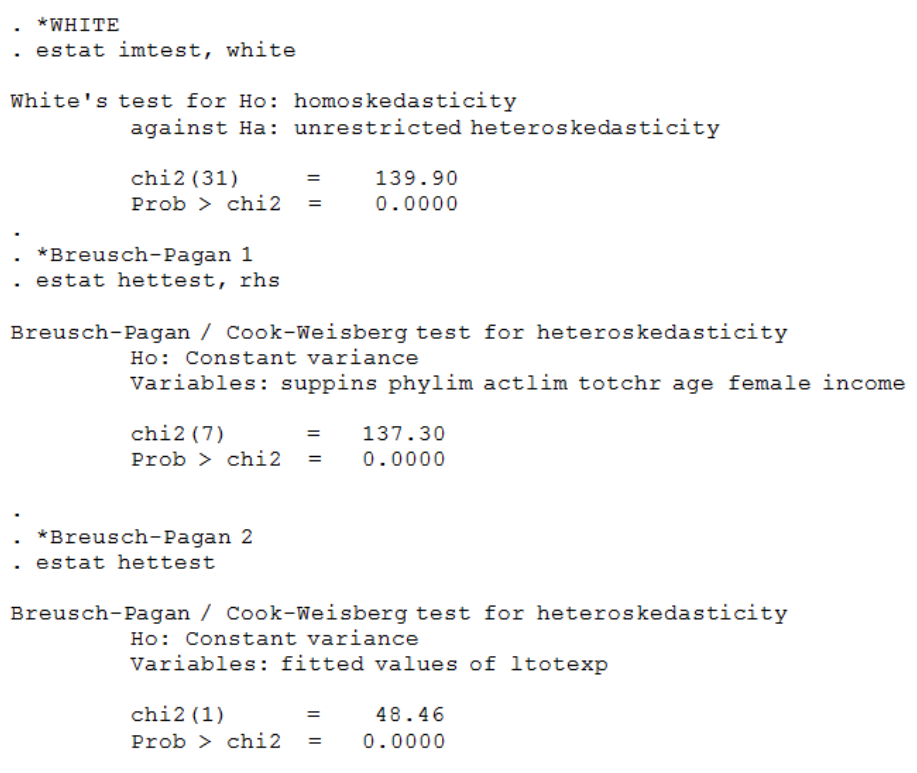
\includegraphics[scale=.37]{fig/stata2b.png}
	\end{figure}
\end{frame}
%---------------------------------------------------
\begin{frame}[fragile]{STATA: Ejemplo 3}
	Consideremos el siguiente conjunto de datos (Fuente: Wooldridge dataset)
{\small
\begin{lstlisting}[language=Stata, numbers=none]
use "http://fmwww.bc.edu/ec-p/data/
wooldridge/MROZ", clear
regress ltotexp suppins phylim actlim totchr age female income
\end{lstlisting}
}
	\begin{figure}
		\centering
		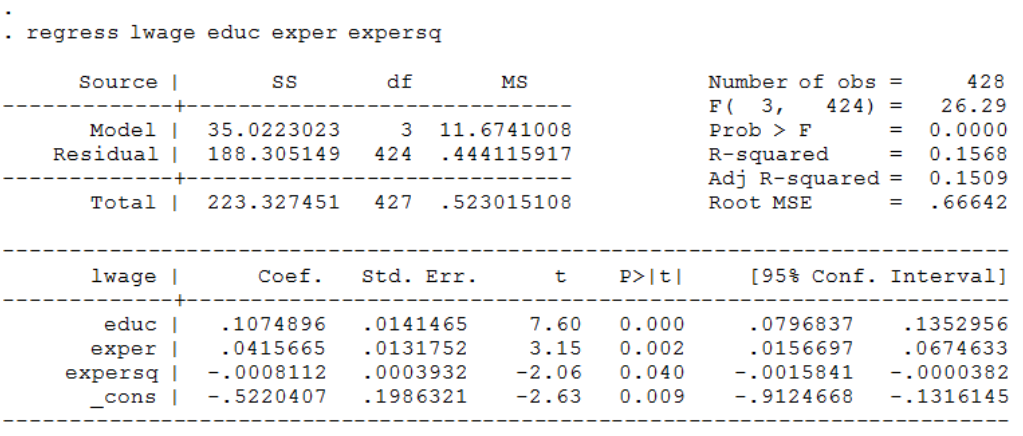
\includegraphics[scale=.35]{fig/stata3a.png}
	\end{figure}
\end{frame}
%---------------------------------------------------
\begin{frame}{STATA: Ejemplo 3}
	\begin{figure}
		\centering
		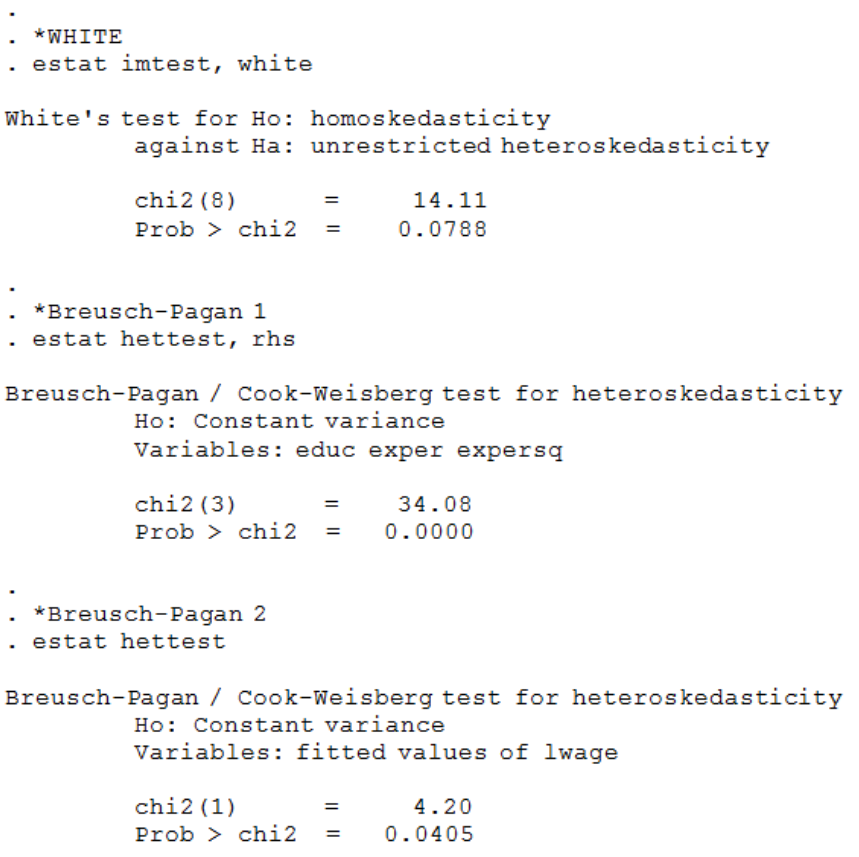
\includegraphics[scale=.36]{fig/stata3b.png}
	\end{figure}
\end{frame}
